% answers.tex —— 2001 年·豫粤卷 · 参考答案与详细解析片段
% 由 tools/generate_projects.py 依来源总账自 2001/2001_数学真题_豫粤_试题.md + 2001/2001_数学真题_豫粤_解析正文.md + 2001/2001_数学真题_豫粤_答案要点.md 生成，勿手改（改源 MD 后重跑）


\begin{gktip}
固定源 PDF 为印刷页码 93–94 的两页题面，不附答案。以下解析均依据题面独立复算；第 11、12、19 题的图形在 LaTeX 工程中以 TikZ/PGFPlots 矢量源重绘。
\end{gktip}

\gkpart{一、选择题}

\begin{answer}
\gksolhead{1}{}

\textbf{题目}：

不等式 $\dfrac{x-1}{x-3}>0$ 的解集为\mbox{（　　）}

（A）$\{x\mid x<1\}$　　（B）$\{x\mid x>3\}$　　（C）$\{x\mid x<1\text{ \text{或} }x>3\}$　　（D）$\{x\mid 1<x<3\}$

\Needspace{4\baselineskip}
\textbf{解析}

\Needspace{5\baselineskip}
临界点为 $x=1,3$。在区间 $(-\infty,1)$ 和 $(3,+\infty)$ 上分子分母同号，故解集为

\nopagebreak[4]
\[
\{x\mid x<1\text{ \text{或} }x>3\},
\]

选 C。

\gkanswer{答案：C}

\end{answer}
\begin{answer}
\gksolhead{2}{}

\textbf{题目}：

若一个圆锥的轴截面是等边三角形，其面积为 $\sqrt3$，则这个圆锥的全面积是\mbox{（　　）}

（A）$3\pi$　　（B）$3\sqrt3\pi$　　（C）$6\pi$　　（D）$9\pi$

\Needspace{4\baselineskip}
\textbf{解析}

\Needspace{5\baselineskip}
设轴截面等边三角形边长为 $\ell$。由面积条件

\nopagebreak[4]
\[
\frac{\sqrt3}{4}\ell^2=\sqrt3
\]

\Needspace{5\baselineskip}
得 $\ell=2$。轴截面底边是圆锥底面直径，所以 $r=1$；轴截面两腰是母线，故 $l=2$。圆锥全面积为

\nopagebreak[4]
\[
S=\pi rl+\pi r^2=2\pi+\pi=3\pi,
\]

选 A。

\gkanswer{答案：A}

\end{answer}
\begin{answer}
\gksolhead{3}{}

\textbf{题目}：

极坐标方程 $\rho^2\cos2\theta=1$ 所表示的曲线是\mbox{（　　）}

（A）两条相交直线　　（B）圆　　（C）椭圆　　（D）双曲线

\Needspace{4\baselineskip}
\textbf{解析}

\Needspace{5\baselineskip}
由极坐标关系 $x=\rho\cos\theta$、$y=\rho\sin\theta$，

\nopagebreak[4]
\[
\rho^2\cos2\theta
=\rho^2(\cos^2\theta-\sin^2\theta)
=x^2-y^2.
\]

\Needspace{5\baselineskip}
所以曲线方程为

\nopagebreak[4]
\[
x^2-y^2=1,
\]

是双曲线，选 D。

\gkanswer{答案：D}

\end{answer}
\begin{answer}
\gksolhead{4}{}

\textbf{题目}：

若定义在区间 $(-1,0)$ 内的函数 $f(x)=\log_{2a}(x+1)$ 满足 $f(x)>0$，则 $a$ 的取值范围是\mbox{（　　）}

（A）$\left(0,\dfrac12\right)$　　（B）$\left(0,\dfrac12\right]$　　（C）$\left(\dfrac12,+\infty\right)$　　（D）$(0,+\infty)$

\Needspace{4\baselineskip}
\textbf{解析}

\Needspace{5\baselineskip}
当 $x\in(-1,0)$ 时，$0<x+1<1$。要使 $\log_{2a}(x+1)>0$，底数必须满足 $0<2a<1$，即

\nopagebreak[4]
\[
0<a<\frac12,
\]

选 A。

\gkanswer{答案：A}

\end{answer}
\begin{answer}
\gksolhead{5}{}

\textbf{题目}：

已知复数 $z=\sqrt2+\sqrt6\,i$，则 $\arg\dfrac1z$ 是\mbox{（　　）}

（A）$\dfrac\pi3$　　（B）$\dfrac{5\pi}3$　　（C）$\dfrac\pi6$　　（D）$\dfrac{11\pi}6$

\Needspace{4\baselineskip}
\textbf{解析}

\Needspace{5\baselineskip}
$z=\sqrt2+\sqrt6\,i$ 位于第一象限，且

\nopagebreak[4]
\[
\tan\arg z=\frac{\sqrt6}{\sqrt2}=\sqrt3,
\]

\Needspace{5\baselineskip}
所以 $\arg z=\pi/3$。因而

\nopagebreak[4]
\[
\arg\frac1z=-\frac\pi3\equiv\frac{5\pi}{3}\pmod{2\pi},
\]

选 B。

\gkanswer{答案：B}

\end{answer}
\begin{answer}
\gksolhead{6}{}

\textbf{题目}：

函数 $y=2^{-x}+1$（$x>0$）的反函数是\mbox{（　　）}

（A）$y=\log_2\dfrac1{x-1}$，$x\in(1,2)$　　（B）$y=-\log_2\dfrac1{x-1}$，$x\in(1,2)$

（C）$y=\log_2\dfrac1{x-1}$，$x\in(1,2]$　　（D）$y=-\log_2\dfrac1{x-1}$，$x\in(1,2]$

\Needspace{4\baselineskip}
\textbf{解析}

\Needspace{5\baselineskip}
由 $y=2^{-x}+1$，得

\nopagebreak[4]
\[
y-1=2^{-x}
\Longrightarrow x=-\log_2(y-1).
\]

\Needspace{5\baselineskip}
交换自变量与因变量，反函数为

\nopagebreak[4]
\[
y=-\log_2(x-1).
\]

原函数的值域为 $(1,2)$，故反函数定义域为 $(1,2)$，选 B。

\gkanswer{答案：B}

\end{answer}
\begin{answer}
\gksolhead{7}{}

\textbf{题目}：

若 $0<\alpha<\beta<\dfrac\pi4$，$\sin\alpha+\cos\alpha=a$，$\sin\beta+\cos\beta=b$，则\mbox{（　　）}

（A）$a>b$　　（B）$a<b$　　（C）$ab<1$　　（D）$ab>2$

\Needspace{4\baselineskip}
\textbf{解析}

\Needspace{5\baselineskip}
令 $h(t)=\sin t+\cos t$。在 $(0,\pi/4)$ 上，

\nopagebreak[4]
\[
h'(t)=\cos t-\sin t>0.
\]

所以 $a=h(\alpha)<h(\beta)=b$，选 B。

\gkanswer{答案：B}

\end{answer}
\begin{answer}
\gksolhead{8}{}

\textbf{题目}：

在正三棱柱 $ABC-A_1B_1C_1$ 中，若 $AB=\sqrt2\,BB_1$，则 $AB_1$ 与 $C_1B$ 所成的角的大小为\mbox{（　　）}

（A）$60^\circ$　　（B）$90^\circ$　　（C）$45^\circ$　　（D）$120^\circ$

\Needspace{4\baselineskip}
\textbf{解析}

\Needspace{5\baselineskip}
设 $BB_1=h$，则 $AB=\sqrt2h$。取正三角形底面坐标

\nopagebreak[4]
\[
A=(0,0,0),\quad B=(\sqrt2h,0,0),\quad
C=\left(\frac{\sqrt2h}{2},\frac{\sqrt6h}{2},0\right),
\]

\Needspace{5\baselineskip}
并令 $A_1,B_1,C_1$ 的 $z$ 坐标均为 $h$。则

\nopagebreak[4]
\[
\overrightarrow{AB_1}=(\sqrt2h,0,h),
\quad
\overrightarrow{C_1B}=\left(\frac{\sqrt2h}{2},-\frac{\sqrt6h}{2},-h\right).
\]

\Needspace{5\baselineskip}
二者数量积为

\nopagebreak[4]
\[
\overrightarrow{AB_1}\cdot\overrightarrow{C_1B}
=h^2-\!h^2=0,
\]

故所成角为 $90^\circ$，选 B。

\gkanswer{答案：B}

\end{answer}
\begin{answer}
\gksolhead{9}{}

\textbf{题目}：

设 $f(x)$、$g(x)$ 都是单调函数，有如下四个命题，其中正确的命题是\mbox{（　　）}

①若 $f(x)$ 单调递增，$g(x)$ 单调递增，则 $f(x)-g(x)$ 单调递增；

②若 $f(x)$ 单调递增，$g(x)$ 单调递减，则 $f(x)-g(x)$ 单调递增；

③若 $f(x)$ 单调递减，$g(x)$ 单调递增，则 $f(x)-g(x)$ 单调递减；

④若 $f(x)$ 单调递减，$g(x)$ 单调递减，则 $f(x)-g(x)$ 单调递减。

（A）①③　　（B）①④　　（C）②③　　（D）②④

\Needspace{4\baselineskip}
\textbf{解析}

递增函数之差不一定递增，递减函数之差也不一定递减，所以①④不恒成立。若 $f$ 递增、$g$ 递减，则 $f-g$ 递增；若 $f$ 递减、$g$ 递增，则 $f-g$ 递减。因此正确的是②③，选 C。

\gkanswer{答案：C}

\end{answer}
\begin{answer}
\gksolhead{10}{}

\textbf{题目}：

对于抛物线 $y^2=4x$ 上任意一点 $Q$，点 $P(a,0)$ 都满足 $|PQ|\ge|a|$，则 $a$ 的取值范围是\mbox{（　　）}

（A）$(-\infty,0)$　　（B）$(-\infty,2]$　　（C）$[0,2]$　　（D）$(0,2)$

\Needspace{4\baselineskip}
\textbf{解析}

\Needspace{5\baselineskip}
抛物线 $y^2=4x$ 上点可表示为

\nopagebreak[4]
\[
Q=(t^2,2t).
\]

\Needspace{5\baselineskip}
于是

\nopagebreak[4]
\[
\begin{aligned}
|PQ|^2-|a|^2
&=(t^2-a)^2+4t^2-a^2\\
&=t^2(t^2+4-2a).
\end{aligned}
\]

要对任意实数 $t$ 非负，必须且只需 $4-2a\ge0$，即 $a\le2$。故 $a\in(-\infty,2]$，选 B。

\gkanswer{答案：B}

\end{answer}
\begin{answer}
\gksolhead{11}{}

\textbf{题目}：

一间民房的屋顶有如图三种不同的盖法：①单向倾斜；②双向倾斜；③四向倾斜。记三种盖法屋顶面积分别为 $P_1$、$P_2$、$P_3$。若屋顶斜面与水平面所成的角都是 $\alpha$，则\mbox{（　　）}
\nopagebreak[4]
\begin{center}% 2001 年豫粤卷第 11 题：三种屋顶盖法
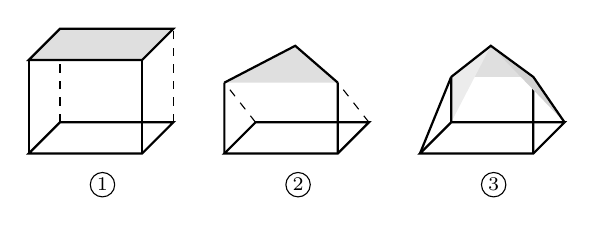
\begin{tikzpicture}[>=stealth, scale=0.72]
  \begin{scope}
    \coordinate (A) at (0,0);
    \coordinate (B) at (2.0,0);
    \coordinate (C) at (2.55,0.55);
    \coordinate (D) at (0.55,0.55);
    \coordinate (A1) at (0,1.65);
    \coordinate (B1) at (2.0,1.65);
    \coordinate (C1) at (2.55,2.2);
    \coordinate (D1) at (0.55,2.2);
    \draw[thick] (A)--(B)--(C)--(D)--cycle;
    \draw[thick] (A)--(A1) (B)--(B1);
    \draw[dashed] (C)--(C1) (D)--(D1);
    \fill[gray!25] (A1)--(B1)--(C1)--(D1)--cycle;
    \draw[thick] (A1)--(B1)--(C1)--(D1)--cycle;
    \node[circle,draw,inner sep=1pt] at (1.3,-0.55) {\scriptsize 1};
  \end{scope}
  \begin{scope}[xshift=3.45cm]
    \coordinate (A) at (0,0);
    \coordinate (B) at (2.0,0);
    \coordinate (C) at (2.55,0.55);
    \coordinate (D) at (0.55,0.55);
    \coordinate (M) at (1.25,1.9);
    \draw[thick] (A)--(B)--(C)--(D)--cycle;
    \draw[thick] (A)--(0,1.25) (B)--(2,1.25);
    \draw[dashed] (C)--(2,1.25) (D)--(0,1.25);
    \fill[gray!25] (0,1.25)--(M)--(2,1.25)--cycle;
    \draw[thick] (0,1.25)--(M)--(2,1.25);
    \node[circle,draw,inner sep=1pt] at (1.3,-0.55) {\scriptsize 2};
  \end{scope}
  \begin{scope}[xshift=6.9cm]
    \coordinate (A) at (0,0);
    \coordinate (B) at (2.0,0);
    \coordinate (C) at (2.55,0.55);
    \coordinate (D) at (0.55,0.55);
    \coordinate (M) at (1.25,1.9);
    \coordinate (L) at (0.55,1.35);
    \coordinate (R) at (2.0,1.35);
    \draw[thick] (A)--(B)--(C)--(D)--cycle;
    \draw[thick] (A)--(L) (B)--(R);
    \draw[dashed] (C)--(R) (D)--(L);
    \fill[gray!25] (L)--(M)--(R)--cycle;
    \fill[gray!15] (D)--(L)--(M)--cycle;
    \fill[gray!35] (M)--(R)--(C)--cycle;
    \draw[thick] (L)--(M)--(R) (D)--(L) (R)--(C);
    \node[circle,draw,inner sep=1pt] at (1.3,-0.55) {\scriptsize 3};
  \end{scope}
\end{tikzpicture}
\end{center}
\nopagebreak[4]
（A）$P_3>P_2>P_1$　　（B）$P_3>P_2=P_1$　　（C）$P_3=P_2>P_1$　　（D）$P_3=P_2=P_1$

\Needspace{4\baselineskip}
\textbf{解析}

\Needspace{5\baselineskip}
把每个屋顶斜面正投影到水平面。斜面与水平面夹角同为 $\alpha$，故斜面面积等于水平投影面积除以 $\cos\alpha$。三种盖法的水平投影区域相同，所以

\nopagebreak[4]
\[
P_1=P_2=P_3,
\]

选 D。

\gkanswer{答案：D}

\end{answer}
\begin{answer}
\gksolhead{12}{}

\textbf{题目}：

如图，小圆圈表示网络的结点，结点之间的连线表示它们有网线相联。连线标注的数字表示该段网线单位时间内可以通过的最大信息量。现从结点 $A$ 向结点 $B$ 传递信息，信息可以分开沿不同的路线同时传递，则单位时间内传递的最大信息量为\mbox{（　　）}
\nopagebreak[4]
\begin{center}% 2001 年豫粤卷第 12 题：信息网络
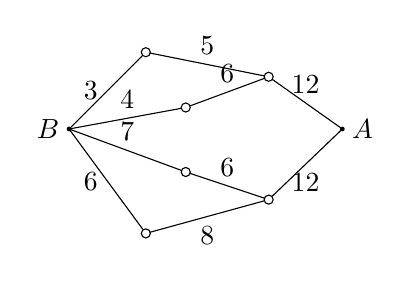
\begin{tikzpicture}[>=stealth, scale=0.78]
  \coordinate (B) at (0,0);
  \coordinate (U) at (1.25,1.25);
  \coordinate (V) at (3.25,0.85);
  \coordinate (M) at (1.9,0.35);
  \coordinate (N) at (1.9,-0.7);
  \coordinate (W) at (1.25,-1.7);
  \coordinate (Z) at (3.25,-1.15);
  \coordinate (A) at (4.45,0);

  \draw (B)--(U) node[midway, left] {3};
  \draw (U)--(V) node[midway, above] {5};
  \draw (B)--(M) node[midway, above] {4};
  \draw (M)--(V) node[midway, above] {6};
  \draw (B)--(N) node[midway, above] {7};
  \draw (N)--(Z) node[midway, above] {6};
  \draw (B)--(W) node[midway, left] {6};
  \draw (W)--(Z) node[midway, below] {8};
  \draw (V)--(A) node[midway, above] {12};
  \draw (Z)--(A) node[midway, below] {12};

  \foreach \point in {U,V,M,N,W,Z}
    \filldraw[fill=white] (\point) circle (2.1pt);
  \fill (B) circle (1.1pt) node[left] {$B$};
  \fill (A) circle (1.1pt) node[right] {$A$};
\end{tikzpicture}
\end{center}
\nopagebreak[4]
（A）$26$　　（B）$24$　　（C）$20$　　（D）$19$

\Needspace{4\baselineskip}
\textbf{解析}

\Needspace{5\baselineskip}
把网络方向反向后，$A$ 到 $B$ 的最大流量不变。上方两条从 $B$ 出发的边容量总和为 $3+4=7$，下方通向 $A$ 的两条边容量总和为 $12+12$，但下方汇流到右下结点时受出口容量 $12$ 限制。因此总流量至多为

\nopagebreak[4]
\[
7+12=19.
\]

上方可取流量 $3+4=7$，下方两条支路各取 $6$，可达到 $19$，故最大信息量为 $19$，选 D。

\gkanswer{答案：D}

\end{answer}
\gkpart{二、填空题}

\begin{answer}
\gksolhead{13}{}

\textbf{题目}：

已知甲、乙两组各有 8 人，现从每组抽取 4 人进行计算机知识竞赛，比赛人员的组成共有\gkblank{}种可能。（用数字作答）

\Needspace{4\baselineskip}
\textbf{解析}

\Needspace{5\baselineskip}
从甲组 8 人中取 4 人、从乙组 8 人中取 4 人，组成数为

\nopagebreak[4]
\[
\binom84\binom84=70^2=4900.
\]

\gkanswer{答案：$4900$}

\end{answer}
\begin{answer}
\gksolhead{14}{}

\textbf{题目}：

双曲线 $\dfrac{x^2}{9}-\dfrac{y^2}{16}=1$ 的两个焦点为 $F_1\text{、}F_2$，点 $P$ 在双曲线上，若 $PF_1\perp PF_2$，则点 $P$ 到 $x$ 轴的距离为\gkblank{}。

\Needspace{4\baselineskip}
\textbf{解析}

\Needspace{5\baselineskip}
双曲线的焦半距为

\nopagebreak[4]
\[
c=\sqrt{9+16}=5,
\]

\Needspace{5\baselineskip}
焦点为 $(\pm5,0)$。设 $P=(x,y)$，因 $PF_1\perp PF_2$，有

\nopagebreak[4]
\[
(x+5,y)\cdot(x-5,y)=0,
\qquad x^2+y^2=25.
\]

\Needspace{5\baselineskip}
又 $P$ 在双曲线上：

\nopagebreak[4]
\[
\frac{x^2}{9}-\frac{y^2}{16}=1.
\]

\Needspace{5\baselineskip}
代入 $x^2=25-y^2$，得

\nopagebreak[4]
\[
\frac{25-y^2}{9}-\frac{y^2}{16}=1
\Longrightarrow y^2=\frac{256}{25}.
\]

\Needspace{5\baselineskip}
所以点 $P$ 到 $x$ 轴的距离为

\nopagebreak[4]
\[
|y|=\frac{16}{5}.
\]

\gkanswer{答案：$\dfrac{16}{5}$}

\end{answer}
\begin{answer}
\gksolhead{15}{}

\textbf{题目}：

设 $\{a_n\}$ 是公比为 $q$ 的等比数列，$S_n$ 是它的前 $n$ 项和。若 $\{S_n\}$ 是等差数列，则 $q=$\gkblank{}。

\Needspace{4\baselineskip}
\textbf{解析}

\Needspace{5\baselineskip}
若 $\{S_n\}$ 为等差数列，则

\nopagebreak[4]
\[
a_{n+1}=S_{n+1}-S_n
\]

为常数。等比数列各项相等时公比为 $1$，故 $q=1$。

\gkanswer{答案：$1$}

\end{answer}
\begin{answer}
\gksolhead{16}{}

\textbf{题目}：

圆周上有 $2n$ 个等分点（$n>1$），以其中三个点为顶点的直角三角形的个数为\gkblank{}。

\Needspace{4\baselineskip}
\textbf{解析}

\Needspace{5\baselineskip}
圆周上的 $2n$ 个等分点两两相对，构成 $n$ 条直径。以任一条直径的两个端点为三角形的两个顶点，再从剩下的 $2n-2$ 个点中选第三点，得到直角三角形；每个直角三角形的斜边直径唯一，因此总数为

\nopagebreak[4]
\[
n(2n-2)=2n(n-1).
\]

\gkanswer{答案：$2n(n-1)$}

\end{answer}
\gkpart{三、解答题}

\begin{answer}
\gksolhead{17}{}

\textbf{题目}：

\Needspace{5\baselineskip}
求函数

\nopagebreak[4]
\[
y=(\sin x+\cos x)^2+2\cos^2x
\]

的最小正周期。

\Needspace{4\baselineskip}
\textbf{解析}

\Needspace{5\baselineskip}
展开并整理：

\nopagebreak[4]
\[
\begin{aligned}
y
&=(\sin x+\cos x)^2+2\cos^2x\\
&=1+\sin2x+1+\cos2x\\
&=2+\sin2x+\cos2x.
\end{aligned}
\]

\Needspace{5\baselineskip}
$\sin2x+\cos2x$ 的最小正周期为 $\pi$，故原函数的最小正周期为

\nopagebreak[4]
\[
\pi.
\]

\gkanswer{答案：$\pi$}

\end{answer}
\begin{answer}
\gksolhead{18}{}

\textbf{题目}：

已知等差数列前三项为 $a,4,3a$，前 $n$ 项的和为 $S_n$，$S_k=2550$。

（1） 求 $a$ 及 $k$ 的值；

\Needspace{5\baselineskip}
（2） 求

\nopagebreak[4]
\[
\lim_{n\to\infty}\left(\frac1{S_1}+\frac1{S_2}+\cdots+\frac1{S_n}\right)
\]

\Needspace{4\baselineskip}
\textbf{解析}

\gksubpart{(1)}

\Needspace{5\baselineskip}
前三项为 $a,4,3a$，等差条件给出

\nopagebreak[4]
\[
4-a=3a-4,
\qquad a=2.
\]

\Needspace{5\baselineskip}
公差 $d=2$，所以

\nopagebreak[4]
\[
S_k=ka+\frac{k(k-1)}2d=k(k+1).
\]

\Needspace{5\baselineskip}
由 $S_k=2550$：

\nopagebreak[4]
\[
k^2+k-2550=0
\Longleftrightarrow (k-50)(k+51)=0.
\]

因 $k$ 为正整数，得 $k=50$。

\gksubpart{(2)}

\Needspace{5\baselineskip}
又 $S_n=n(n+1)$，故

\nopagebreak[4]
\[
\sum_{j=1}^n\frac1{S_j}
=\sum_{j=1}^n\frac1{j(j+1)}
=1-\frac1{n+1}.
\]

所以极限为 $1$。

\gkanswer{答案（1）：$a=2,\ k=50$。}

\gkanswer{答案（2）：$1$。}

\end{answer}
\begin{answer}
\gksolhead{19}{}

\textbf{题目}：

如图，在底面是直角梯形的四棱锥 $S-ABCD$ 中，$\angle ABC=90^\circ$，$SA\perp$ 面 $ABCD$，$SA=AB=BC=1$，$AD=\dfrac12$。
\nopagebreak[4]
\begin{center}% 2001 年豫粤卷第 19 题：直角梯形底面的四棱锥
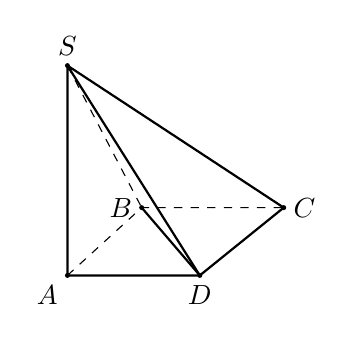
\begin{tikzpicture}[>=stealth, scale=0.82]
  \coordinate (A) at (0,0);
  \coordinate (B) at (1.15,1.05);
  \coordinate (C) at (3.35,1.05);
  \coordinate (D) at (2.05,0);
  \coordinate (S) at (0,3.25);

  \draw[thick] (S)--(A) (S)--(C) (S)--(D);
  \draw[dashed] (S)--(B);
  \draw[thick] (A)--(D)--(C);
  \draw[dashed] (A)--(B)--(C);
  \draw[thick] (B)--(D);

  \fill (S) circle (1.1pt) node[above] {$S$};
  \fill (A) circle (1.1pt) node[below left] {$A$};
  \fill (B) circle (1.1pt) node[left] {$B$};
  \fill (C) circle (1.1pt) node[right] {$C$};
  \fill (D) circle (1.1pt) node[below] {$D$};
\end{tikzpicture}
\end{center}
\nopagebreak[4]
（1） 求四棱锥 $S-ABCD$ 的体积；

（2） 求面 $SCD$ 与面 $SBA$ 所成的二面角的正切值。

\Needspace{4\baselineskip}
\textbf{解析}

\gksubpart{(1)}

\Needspace{5\baselineskip}
底面直角梯形面积为

\nopagebreak[4]
\[
S_{ABCD}=\frac{(BC+AD)\cdot AB}{2}
=\frac{(1+1/2)\cdot1}{2}
=\frac34.
\]

\Needspace{5\baselineskip}
因 $SA$ 垂直底面且 $SA=1$，四棱锥体积为

\nopagebreak[4]
\[
V=\frac13S_{ABCD}\cdot SA=\frac14.
\]

\gksubpart{(2)}

\Needspace{5\baselineskip}
延长 $BA$、$CD$ 相交于 $E$，连接 $SE$，则 $SE$ 是所求二面角的棱。由于 $AD\parallel BC$ 且 $BC=2AD$，可得 $EA=AB=SA=1$。在直角三角形 $SAB$ 中，

\nopagebreak[4]
\[
SB=\sqrt{SA^2+AB^2}=\sqrt2.
\]

\Needspace{5\baselineskip}
又 $BC\perp SB$，所以二面角的平面角 $\varphi$ 满足

\nopagebreak[4]
\[
\tan\varphi=\frac{BC}{SB}=\frac1{\sqrt2}=\frac{\sqrt2}{2}.
\]

\gkanswer{答案（1）：$\dfrac14$。}

\gkanswer{答案（2）：$\dfrac{\sqrt2}{2}$。}

\end{answer}
\begin{answer}
\gksolhead{20}{}

\textbf{题目}：

设计一幅宣传画，要求画面面积为 $4840\ \mathrm{cm}^2$，画面的宽与高的比为 $\lambda$（$\lambda<1$），画面的上、下各留 $8\ \mathrm{cm}$ 空白，左、右各留 $5\ \mathrm{cm}$ 空白。怎样确定画面的高与宽尺寸，能使宣传画所用纸张的面积最小？如果要求 $\lambda\in\left[\dfrac23,\dfrac34\right]$，那么 $\lambda$ 为何值时，能使宣传画所用纸张的面积最小？

\Needspace{4\baselineskip}
\textbf{解析}

\Needspace{5\baselineskip}
设画面高为 $x$ cm，宽为 $\lambda x$ cm。由画面面积，

\nopagebreak[4]
\[
\lambda x^2=4840.
\]

\Needspace{5\baselineskip}
纸张面积为

\nopagebreak[4]
\[
\begin{aligned}
S
&=(x+16)(\lambda x+10)\\
&=5000+10x+\frac{77440}{x}\\
&=5000+44\sqrt{10}\left(8\sqrt\lambda+\frac5{\sqrt\lambda}\right).
\end{aligned}
\]

\Needspace{5\baselineskip}
对第一问，$\lambda=4840/x^2$，所以

\nopagebreak[4]
\[
S=5000+10x+\frac{77440}{x}.
\]

\Needspace{5\baselineskip}
由基本不等式，$S$ 在 $10x=77440/x$ 时取得最小值，即 $x=88$。此时

\nopagebreak[4]
\[
\lambda=\frac{4840}{88^2}=\frac58,\qquad
\lambda x=55.
\]

故第一问画面高为 $88\ \mathrm{cm}$、宽为 $55\ \mathrm{cm}$。

\Needspace{5\baselineskip}
对第二问，在给定 $\lambda$ 下有

\nopagebreak[4]
\[
x=\frac{22\sqrt{10}}{\sqrt\lambda},
\qquad
\lambda x=22\sqrt{10\lambda},
\]

\Needspace{5\baselineskip}
纸张面积可写为

\nopagebreak[4]
\[
S=5000+44\sqrt{10}\left(8\sqrt\lambda+\frac5{\sqrt\lambda}\right).
\]

\Needspace{5\baselineskip}
令 $t=\sqrt\lambda$，则需在 $t\in[\sqrt{2/3},\sqrt{3/4}]$ 上考察

\nopagebreak[4]
\[
8t+\frac5t.
\]

\Needspace{5\baselineskip}
其导数为 $8-5/t^2$；无约束极小点满足 $t^2=5/8$，即 $\lambda=5/8$，但不在 $\left[2/3,3/4\right]$ 内。区间内 $t^2>5/8$，函数递增，因此最小值在左端取得：

\nopagebreak[4]
\[
\lambda=\frac23.
\]

\gkanswer{答案：第一问画面高为 $88\ \mathrm{cm}$、宽为 $55\ \mathrm{cm}$（此时 $\lambda=\dfrac58$）；第二问当 $\lambda\in\left[\dfrac23,\dfrac34\right]$ 时取 $\lambda=\dfrac23$。}

\end{answer}
\begin{answer}
\gksolhead{21}{}

\textbf{题目}：

已知椭圆 $\dfrac{x^2}{4}+y^2=1$ 的右准线 $l$ 与 $x$ 轴相交于点 $E$，过椭圆右焦点 $F$ 的直线与椭圆相交于 $A\text{、}B$ 两点，点 $C$ 在右准线 $l$ 上，且 $BC\perp x$ 轴，求证：直线 $AC$ 经过线段 $EF$ 的中点。

\Needspace{4\baselineskip}
\textbf{解析}

\Needspace{5\baselineskip}
椭圆

\nopagebreak[4]
\[
\frac{x^2}{4}+y^2=1
\]

\Needspace{5\baselineskip}
的半长轴 $a_0=2$、半焦距 $c_0=\sqrt3$，右焦点为 $F=(\sqrt3,0)$，右准线为

\nopagebreak[4]
\[
l:\ x=\frac{a_0^2}{c_0}=\frac4{\sqrt3}.
\]

\Needspace{5\baselineskip}
故 $E=(4/\sqrt3,0)$。设过 $F$ 的直线斜率为 $m$，与椭圆交于 $A(x_A,y_A)$、$B(x_B,y_B)$，则

\nopagebreak[4]
\[
y=m(x-\sqrt3).
\]

\Needspace{5\baselineskip}
把它代入椭圆方程，得到关于交点横坐标的二次方程

\nopagebreak[4]
\[
(1+4m^2)x^2-8\sqrt3m^2x+12m^2-4=0.
\]

\Needspace{5\baselineskip}
由韦达定理，

\nopagebreak[4]
\[
x_A+x_B=\frac{8\sqrt3m^2}{1+4m^2},
\qquad
x_Ax_B=\frac{12m^2-4}{1+4m^2}.
\]

\Needspace{5\baselineskip}
点 $C$ 在右准线上且 $BC\perp x$ 轴，所以

\nopagebreak[4]
\[
C=\left(\frac4{\sqrt3},y_B\right).
\]

\Needspace{5\baselineskip}
设 $M$ 为 $EF$ 的中点，则

\nopagebreak[4]
\[
M=\left(\frac7{2\sqrt3},0\right).
\]

\Needspace{5\baselineskip}
直线 $AC$ 与 $x$ 轴交点的横坐标为

\nopagebreak[4]
\[
\frac{x_Ay_B-\frac4{\sqrt3}y_A}{y_B-y_A}.
\]

\Needspace{5\baselineskip}
代入 $y_A=m(x_A-\sqrt3)$、$y_B=m(x_B-\sqrt3)$，并利用韦达关系，分子可整理为

\nopagebreak[4]
\[
x_Ax_B-\frac7{\sqrt3}x_A+4.
\]

\Needspace{5\baselineskip}
另一方面，

\nopagebreak[4]
\[
\frac7{2\sqrt3}(x_B-x_A)
=\frac7{2\sqrt3}(x_A+x_B-2x_A).
\]

\Needspace{5\baselineskip}
由

\nopagebreak[4]
\[
x_Ax_B+4=\frac7{2\sqrt3}(x_A+x_B),
\]

二者相等，所以直线 $AC$ 与 $x$ 轴交于 $M$，即 $AC$ 经过线段 $EF$ 的中点。

\gkanswer{答案：见解析。}

\end{answer}
\begin{answer}
\gksolhead{22}{}

\textbf{题目}：

设 $f(x)$ 是定义在 $\mathbb R$ 上的偶函数，其图象关于直线 $x=1$ 对称，对任意 $x_1,x_2\in\left[0,\dfrac12\right]$，都有 $f(x_1+x_2)=f(x_1)\cdot f(x_2)$，且 $f(1)=a>0$。

（1） 求 $f\left(\dfrac12\right),f\left(\dfrac14\right)$；

（2） 证明：$f(x)$ 是周期函数；

（3） 记 $a_n=f\left(2n+\dfrac1{2n}\right)$，求 $\displaystyle\lim_{n\to\infty}\ln a_n$。

\Needspace{4\baselineskip}
\textbf{解析}

\Needspace{5\baselineskip}
由偶函数性质和图象关于 $x=1$ 对称，分别有

\nopagebreak[4]
\[
f(-x)=f(x),\qquad f(2-x)=f(x).
\]

\gksubpart{(1)}

\Needspace{5\baselineskip}
由乘法条件，

\nopagebreak[4]
\[
f(1)=f\left(\frac12+\frac12\right)
=f\left(\frac12\right)^2=a.
\]

\Needspace{5\baselineskip}
结合 $a>0$ 及同样的平方关系，可取正根，得

\nopagebreak[4]
\[
f\left(\frac12\right)=\sqrt a.
\]

\Needspace{5\baselineskip}
再由

\nopagebreak[4]
\[
f\left(\frac12\right)
=f\left(\frac14+\frac14\right)
=f\left(\frac14\right)^2,
\]

\Needspace{5\baselineskip}
得

\nopagebreak[4]
\[
f\left(\frac14\right)=\sqrt[4]a.
\]

\gksubpart{(2)}

\Needspace{5\baselineskip}
由对称性

\nopagebreak[4]
\[
f(x)=f(2-x)=f(x-2),
\]

其中第二步使用了偶性。因此 $2$ 是 $f(x)$ 的一个周期。

\gksubpart{(3)}

\Needspace{5\baselineskip}
先由周期性，

\nopagebreak[4]
\[
a_n=f\left(2n+\frac1{2n}\right)
=f\left(\frac1{2n}\right).
\]

\Needspace{5\baselineskip}
将 $1/(2n)$ 连加 $n$ 次，并逐步使用题设乘法关系，可得

\nopagebreak[4]
\[
f\left(\frac1{2n}\right)^n=f\left(\frac12\right)=\sqrt a.
\]

\Needspace{5\baselineskip}
所以

\nopagebreak[4]
\[
a_n=f\left(\frac1{2n}\right)=a^{1/(2n)},
\qquad
\ln a_n=\frac{\ln a}{2n}\longrightarrow0.
\]

\gkanswer{答案（1）：$f\left(\dfrac12\right)=\sqrt a,\ f\left(\dfrac14\right)=\sqrt[4]a$。}

\gkanswer{答案（2）：$f(x)$ 的一个周期为 $2$。}

\gkanswer{答案（3）：$0$。}

\end{answer}